%%%%%%%%%%%%%%%%%%%%%%%%%%%%%%%%%%%%%%%%%%%%%%%%%%%%%%%%%%%%%%%%%%%%%%%%%%%%%%%%%%%%%%%%%%%
% LaTeX Template of the Chair of Enterprise Systems
% Version 0.92
% Author: Marcel-René Wepper
% Questions? Feedback? Remarks? -> marce-rene.wepper@uni-mannheim.de
%%%%%%%%%%%%%%%%%%%%%%%%%%%%%%%%%%%%%%%%%%%%%%%%%%%%%%%%%%%%%%%%%%%%%%%%%%%%%%%%%%%%%%%%%%%

%%%%%%%%%%%%%%%%%%%%%%%%%%%%%%%%%%%%%%%%%%%%%%%%%%%%%%%%%%%%%%%%%%%%%%%%%%%%%%%%%%%%%%%%%%%
% !!! IMPORTANT !!!
% 1) Use/upload whole template folder, including "fonts" and "images" subfolder
%    e.g Overleaf: "upload" (top-left) -> Select all contents of template folder
% 2) Make sure XeLaTeX is selected as Latex Compiler 
%    e.g Overleaf: "Menu" (top-left) -> Compiler -> Select "XeLaTeX"
% 3) Make sure 
%    e.g Overleaf: "Menu" (top-left) -> Main document -> Select "main.tex
%%%%%%%%%%%%%%%%%%%%%%%%%%%%%%%%%%%%%%%%%%%%%%%%%%%%%%%%%%%%%%%%%%%%%%%%%%%%%%%%%%%%%%%%%%%

%%%%%%%%%%%%%%%%%%%%%%%%%%%%%%%%%%%%%%%%%%%%%%%%%%%%%%%%%%%%%%%%%%%%%%%%%%%%%%%%%%%%%%%%%%%
% Changelog
% 0.92 Made it work for 2023 XeLaTeX
% 0.91 Switched bibliography backend from biber to bibtex (Thanks to Fareed! :-)
%%%%%%%%%%%%%%%%%%%%%%%%%%%%%%%%%%%%%%%%%%%%%%%%%%%%%%%%%%%%%%%%%%%%%%%%%%%%%%%%%%%%%%%%%%%


\input{settings.tex}
\xpatchbibmacro{date+extradate}{%
  \printtext[parens]%
}{%
  \setunit{\addperiod\space}%
  \printtext%
}{}{}

\DeclareDelimFormat[bib,biblist]{nametitledelim}{.\space}

%%%%%%%%%%%%%%%%%%%%%%%%%%%%%%%%%%%%%%%%%%%%%%%%%%%%%%%%%%%%%%%%%%%%%%%%%%%%%%%%%%%%%%%%%%%
% "Title Page" Section
%%%%%%%%%%%%%%%%%%%%%%%%%%%%%%%%%%%%%%%%%%%%%%%%%%%%%%%%%%%%%%%%%%%%%%%%%%%%%%%%%%%%%%%%%%%



\begin{document}
\newtheorem{definition}{Definition}[section]

\begin{titlepage}
	\centering

    
\includegraphics[width=7.38cm]{logo_university_of_mannheim.png}\par

	\vspace{1.25cm}
	{\scshape\Large\uppercase{The Role of Gender Equality Contexts in Women’s Tech Careers: 
	A Quantitative Cross-Country Comparison of Low-Code/No-Code and Traditional Development Roles}}
	
	\vspace{3cm}
	{\linespread{1}\normalsize Master Thesis\\
	 of  \par}
	
	{\large \fauxsc{Carolin Rabe}\par}
	
	\vspace{0.5cm}
%	{\small \titledate\today \par} % uncomment this line use date of today automatically
	{\small 31. July 2026 \par} %
	
	\vspace{0.3cm}
	{\footnotesize  Matriculation Number\\
	2032910\par}
	
	\vspace{2cm}
	\hrulefill\\	
	\vspace{1.0cm}
	{\linespread{1}\normalsize Submitted at the Chair of Enterprise Systems\\
	University of Mannheim\par}
	
	\vspace{0.3cm}
	{\linespread{1}\normalsize  Reviewer: Marcel-René Wepper \\ \par}
	% Supervisor: Name Last-name \par}


\end{titlepage}
\centering
\pagenumbering{gobble}


\vspace{2.5cm}

\newpage
\renewcommand{\contentsname}{Table of Contents} % table of content heading


%%%%%%%%%%%%%%%%%%%%%%%%%%%%%%%%%%%%%%%%%%%%%%%%%%%%%%%%%%%%%%%%%%%%%%%%%%%%%%%%%%%%%%%%%%%
% "Table of Content", "List of Figures", "List of Tables" Section
\newgeometry{top=3cm,bottom=2cm,right=3cm,left=3cm} % update page margins
%%%%%%%%%%%%%%%%%%%%%%%%%%%%%%%%%%%%%%%%%%%%%%%%%%%%%%%%%%%%%%%%%%%%%%%%%%%%%%%%%%%%%%%%%%%

\pagenumbering{roman} % set capital roman page numbers: I, II, ...
\clearpage \setcounter{page}{2} % count cover page
\tableofcontents

\newpage
\addcontentsline{toc}{section}{\listfigurename}
\listoffigures

\newpage
\addcontentsline{toc}{section}{\listtablename}
\listoftables
\newpage



%%%%%%%%%%%%%%%%%%%%%%%%%%%%%%%%%%%%%%%%%%%%%%%%%%%%%%%%%%%%%%%%%%%%%%%%%%%%%%%%%%%%%%%%%%%
% "Abbreviations" Section 
%%%%%%%%%%%%%%%%%%%%%%%%%%%%%%%%%%%%%%%%%%%%%%%%%%%%%%%%%%%%%%%%%%%%%%%%%%%%%%%%%%%%%%%%%%%


\nomenclature[A]{\textbf{tbd.}}{To Be Done}

% Avoid warning when nomenclature index was not generated yet.
\IfFileExists{main.nls}{\printnomenclature[7cm]}{}
\addcontentsline{toc}{section}{List of Abbreviations}
\newpage

%%%%%%%%%%%%%%%%%%%%%%%%%%%%%%%%%%%%%%%%%%%%%%%%%%%%%%%%%%%%%%%%%%%%%%%%%%%%%%%%%%%%%%%%%%%
% "Abstract" Section
%%%%%%%%%%%%%%%%%%%%%%%%%%%%%%%%%%%%%%%%%%%%%%%%%%%%%%%%%%%%%%%%%%%%%%%%%%%%%%%%%%%%%%%%%%%
\justifying
\sectionunnumbered{Abstract}

Lorem Ipsum...
\newpage

%%%%%%%%%%%%%%%%%%%%%%%%%%%%%%%%%%%%%%%%%%%%%%%%%%%%%%%%%%%%%%%%%%%%%%%%%%%%%%%%%%%%%%%%%%%
% "Main Document" Section
\pagenumbering{arabic} % set capital roman page numbers: 1,2,...
%%%%%%%%%%%%%%%%%%%%%%%%%%%%%%%%%%%%%%%%%%%%%%%%%%%%%%%%%%%%%%%%%%%%%%%%%%%%%%%%%%%%%%%%%%%
\newpage
\section{Introduction}
\subsection{Background Gender Equality in Technology Sector}
\subsection{Background Low-Code /No-Code Development Platforms}
\subsection{Research Problem and Analytical Gap}
\subsection{Research Objectives and Questions}
\subsection{Structure of the Thesis}

Lorem Ipsum...

\begin{table}[!ht]
\centering
\begin{tabularx}{\textwidth}{|X|}
\hline
\multicolumn{1}{|c|}{\textbf{ Hypotheses}}\\ \hline
1. Hypo 1 \\ \hline
2. Hypo 2 \\ \hline
3. Hypo 3 \\ \hline
\end{tabularx}
\caption{Final Hypotheses}
\label{tab:hypo}
\end{table}

Table \ref{tab:hypo} shows the final hypotheses.

\begin{figure}[H]
\centering
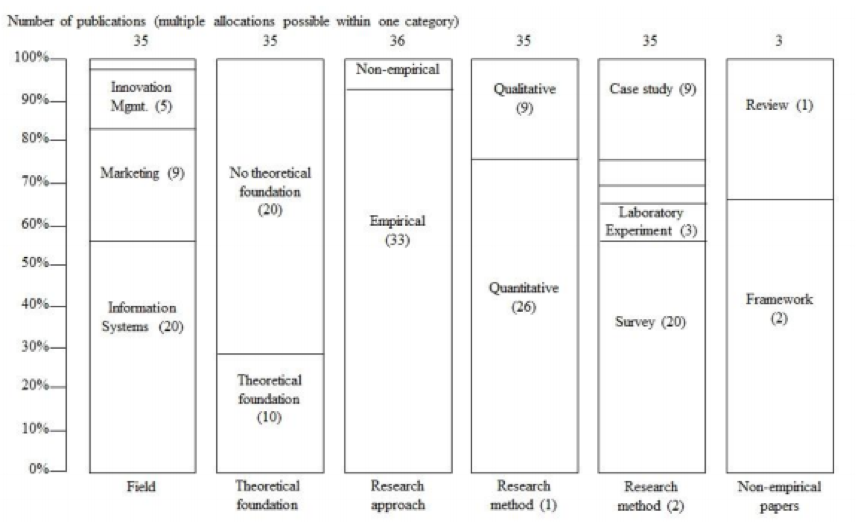
\includegraphics[width=1.0\textwidth]{images/Picture1.png}
\caption{Number of Publications} % \cite{teichert_machine_2019}}
\label{fig:nop}
\end{figure}

Figure \ref{fig:nop} shows the number of publications. 
\include{chapters/2_Theoretical_Background}
\include{chapters/3_Research_Design}
\include{chapters/4_Results}
\include{chapters/5_Discussion}
\include{chapters/6_Conclusion}	

%%%%%%%%%%%%%%%%%%%%%%%%%%%%%%%%%%%%%%%%%%%%%%%%%%%%%%%%%%%%%%%%%%%%%%%%%%%%%%%%%%%%%%%%%%%
% "Bibliography" Section
% IMPORTANT: Do not change anything here!
% Add/change your bibliography entries to the "bibliography.bib" file
% Remark: Entries only show up in this section, after you \cite them at least once.
%%%%%%%%%%%%%%%%%%%%%%%%%%%%%%%%%%%%%%%%%%%%%%%%%%%%%%%%%%%%%%%%%%%%%%%%%%%%%%%%%%%%%%%%%%%

\sectionunnumbered{Bibliography}
\pagenumbering{Roman} % set roman page numbers: i, ii, ...
{\linespread{1}\selectfont\printbibliography[heading=none]}

 \newpage

%%%%%%%%%%%%%%%%%%%%%%%%%%%%%%%%%%%%%%%%%%%%%%%%%%%%%%%%%%%%%%%%%%%%%%%%%%%%%%%%%%%%%%%%%%%
% "Appendix" Section
%%%%%%%%%%%%%%%%%%%%%%%%%%%%%%%%%%%%%%%%%%%%%%%%%%%%%%%%%%%%%%%%%%%%%%%%%%%%%%%%%%%%%%%%%%%

\sectionunnumbered{Appendix}

This appendix section is currently a placeholder.


%%%%%%%%%%%%%%%%%%%%%%%%%%%%%%%%%%%%%%%%%%%%%%%%%%%%%%%%%%%%%%%%%%%%%%%%%%%%%%%%%%%%%%%%%%%
% "Affidavit" Section
%%%%%%%%%%%%%%%%%%%%%%%%%%%%%%%%%%%%%%%%%%%%%%%%%%%%%%%%%%%%%%%%%%%%%%%%%%%%%%%%%%%%%%%%%%%

\sectionunnumbered{Statement about Generative AI or Large Language Model Use}
% Here you should shortly outline how you used generative AI or large language models, e.g., OpenAI’s ChatGPT or Meta’s Llama, for writing your thesis. This encompasses all stages like finding a topic, literature search, analysis, or writing. Please note that employing these models as support is allowed while it is not allowed to employ them like a ghostwriter. For detailed information on this, please refer to the information provided by the Chair. Furthermore, you may be asked to hand in your complete chat history with any model pertaining to your thesis digitally as PDF. Eventually, you find helpful information on this matter in this document provided by the university: https://www.uni-mannheim.de/media/Einrichtungen/Koordinationsstelle_Studieninformationen/Dokumente/Erstsemester/ChatGPT_Handreichung_Studierende_UMA_Stand_Mai_2023.pdf 

\sectionunnumbered{Affidavit} 
{I hereby declare that I have developed and written the enclosed Master thesis entirely on my own and have not used outside sources without declaration in the text. Any concepts or quotations applicable to these sources are clearly attributed to them.\par}
\vspace{0.7cm}
{This Master thesis has not been submitted in the same or substantially similar version, not even in part, to any other authority for grading and has not been published elsewhere. I am aware of the fact that a misstatement may have serious legal consequences.\par}
\vspace{0.7cm}

%Mannheim,  \titledate\today %  uncomment this line use date of today automatically

\vspace{0.5cm}
\begin{table}[h]
\raggedright
\setlength{\extrarowheight}{.5em}
\begin{tabular}{ll}
Date:               & XX.XX.XXXX                       \\
Name of Student:    & XXXXXX XXXXXX               \\
Address of Student: & XXXXXX XXXXXX  
\end{tabular}
\end{table}

\vspace{2.5cm}
\begin{table}[h]
\raggedright
\begin{tabular}{@{}p{.65in}p{2.25in}@{}}
Signature: & \hrulefill
\end{tabular}
\end{table}


\end{document}
